\documentclass{beamer}

\mode<presentation>
{
  \usetheme{Frankfurt}
  \usecolortheme{orchid}
  \setbeamercovered{invisible}
  \setbeamertemplate{footline}[frame number]
}

\usepackage[english]{babel}
\usepackage[latin1]{inputenc}
\usepackage{times}
\usepackage[T1]{fontenc}
\usepackage{tikz}
\usepackage{array}
\usepackage{cancel}


\usetikzlibrary{shapes,backgrounds}

\def\multiset#1#2{\ensuremath{\left(\kern-.3em\left(\genfrac{}{}{0pt}{}{#1}{#2}\right)\kern-.3em\right)}}

\def\blue{\color{blue}~}
\def\black{\color{black}~}
\def\bl[#1]#2{\begin{block}{#1}#2\end{block}}
\def\integers{\mathbb{Z}}
\def\enumb{\begin{enumerate}}
\def\enume{\end{enumerate}}
\def\itemb{\begin{itemize}}
\def\iteme{\end{itemize}}
\def\div{~\textrm{div}~}
\def\mod{~\textrm{mod}~}


\usepackage{remreset}
\makeatletter
\@removefromreset{subsection}{section}
\makeatother
\setcounter{subsection}{1}

\title{Discrete Mathematics, Section 002, Spring 2016}
\subtitle{Lecture 24: Simple graphs and their subgraphs}

\author[Zsolt]{Zsolt Pajor-Gyulai \\ \texttt{zsolt@cims.nyu.edu}}

\pgfdeclareimage[height=1cm]{NYUlogo}{NYUlogo.jpg}

\institute[NYU] 
{
\normalsize Courant Institute of Mathematical Sciences
}
\titlegraphic{\pgfuseimage{NYUlogo}}

\begin{document}

\begin{frame}
  \titlepage
\end{frame}

\AtBeginSection[]
{
\begin{frame}
\frametitle{Outline}
\tableofcontents[currentsection]
\end{frame}}

\section{Motivating examples}

\begin{frame}{Map coloring}
\begin{columns}
\column{0.5\textwidth}
\only<1>{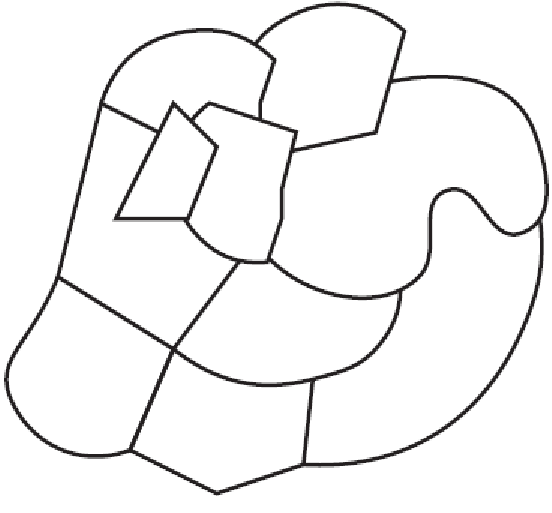
\includegraphics[scale=0.5]{Emptymap.pdf}}
\only<2->{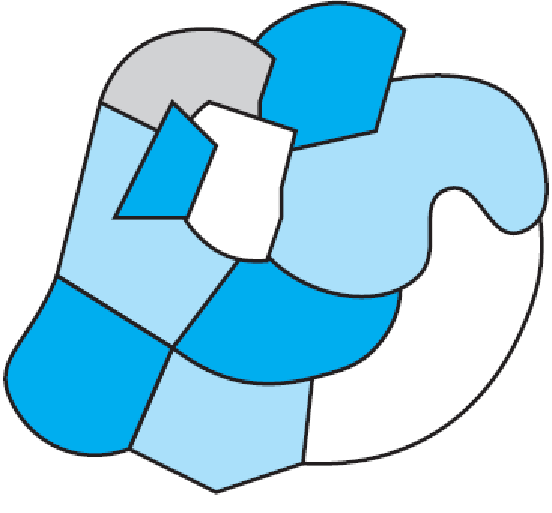
\includegraphics[scale=0.5]{Coloredmap.pdf}}
\column{0.5\textwidth}
How many colors do you need to color a map such that bordering countries have different colors?

\end{columns}
\uncover<3->{
\itemb
\item Can this map be colored with fewer than four colors?\uncover<4->{$~~~\to\textrm{No}$}
\item Is there another map that can be colored with fewer than four colors?\uncover<4->{$~~~\to\textrm{Yes}$}
\item Is there a map that requires more than four colors?\uncover<4->{$~~~\to\textrm{No}$}
\iteme}
\end{frame}

\begin{frame}{Map coloring $\to$ scheduling}
\underline{If you think map coloring is useless:}\vspace{0.8cm}

Assume a university has a lot of students and a lot of courses. How many exams does a university need to hold so that nobody has a conflict.

\begin{figure}
\center
\begin{tabular}{|r|l|l|}
\hline
\textcolor{blue}{Problem}&\textcolor{blue}{Map Coloring}&\textcolor{blue}{Exam scheduling}\\
\hline
\hline
\textrm{Assign}&\textrm{colors}&\textrm{time slots}\\
\textrm{to}&\textrm{countries}&\textrm{courses}\\
\textrm{condition}&\textrm{common border}&\textrm{common student} \\
&$\Rightarrow$ \textrm{different colors}&$\Rightarrow$ \textrm{different slots}\\
\textrm{objective}&\textrm{fewest color}&\textrm{fewest time slots}\\
\hline
\end{tabular}
\end{figure}
\end{frame}

\begin{frame}{Three utilities}
\begin{columns}
\column{0.5\textwidth}
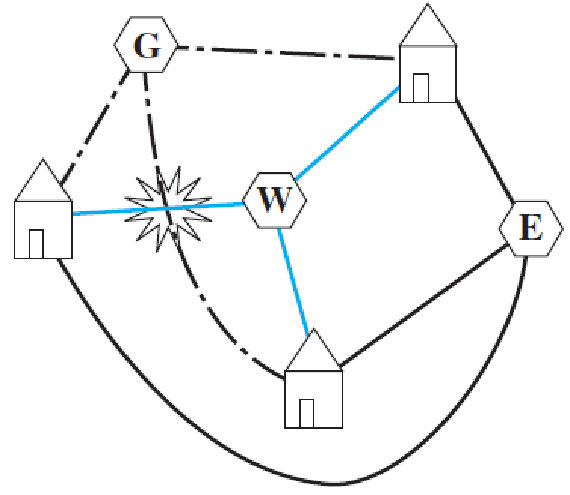
\includegraphics[scale=0.45]{ThreeUtils.pdf}
\column{0.5\textwidth}
Gas-Electric-Water needs to be connected to all houses and pipes cannot cross.\vspace{0.5cm}

\center \color{red} This is not possible!
\end{columns}\vspace{0.3cm}
\underline{If you think this is silly:}
\vspace{0.5cm}

On a printed circuit board, resistors, capacitors, etc. are printed on a flat piece of plastic. Connections between these are by printing metal wires on the surface. If two crossed, that would be short circuit and one has to use multi-layers which are expensive.
\end{frame}

\begin{frame}{Seven bridges}
\begin{columns}
\column{0.5\textwidth}
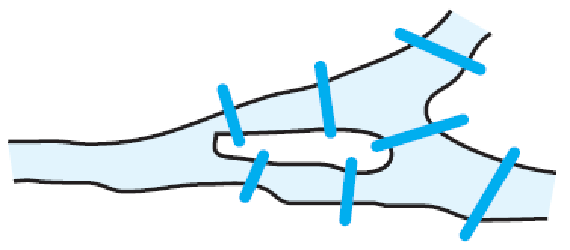
\includegraphics[scale=0.45]{7bridges.pdf}
\column{0.5\textwidth}
Is there a tour of the city we can take through so that we cross every bridge exactly once?\vspace{0.5cm}

\center \color{red} This is not possible!
\end{columns}\vspace{0.3cm}
\underline{If you think this is silly:}
\vspace{0.5cm}

Think about organizing garbage collection in the city and optimizing the path of the garbage truck.
\end{frame}

\section{Simple graphs}

\begin{frame}{Definition of a simple graph}
\bl[Definition]{
A \textbf{simple graph} is a pair $G=(V,E)$ where $V$ is a nonempty finite set and $E$ is a set of two element subsets of $V$
}
For example,
\[
G=(\{1,2,3,4,5,6,7\},\left\{\{1,2\}, \{1,3\},\{2,3\},\{3,4\},\{5,6\}\right\})
\]
Here
\[
V=\{1,2,3,4,5,6,7\}\qquad E=\left\{\{1,2\}, \{1,3\},\{2,3\},\{3,4\},\{5,6\}\right\}
\]\vspace{-0.3cm}
\bl[Terminology]{
The elements of $V$ are called \textbf{vertices} (singular: vertex), and the elements of $E$ are called \textbf{edges}.
}
\end{frame}

\begin{frame}{Visualization of a simple graph}\vspace{-0.5cm}
\[
G=(\{1,2,3,4,5,6,7\},\left\{\{1,2\}, \{1,3\},\{2,3\},\{3,4\},\{5,6\}\right\})
\]\vspace{-0.4cm}\\
\itemb
\item For every $v\in V$, draw a node.
\item For every $e\in E$, draw a line connecting 
\[
v_i,v_j\in V\qquad\textrm{where}\qquad e=\{v_i,v_j\}.
\]
\iteme
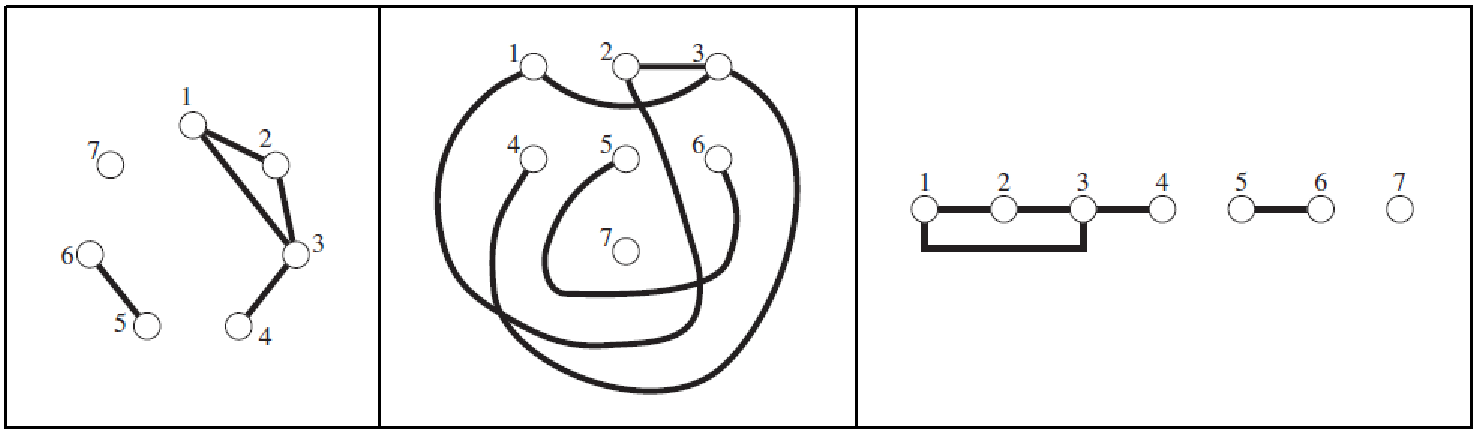
\includegraphics[scale=0.45]{ExampleVisual.pdf}

All three are all good visualizations of $G$ however the left and rightmost are obviously clearer. (Do Problems 1-2 on WS)
\end{frame}

\begin{frame}{Warnings}
\itemb
\item $e\in E$ is a two element set.
\item Therefore an edge cannot be $\{u,u\}$ (No loops.)
\item No parallel edges either.
\iteme

\center{This is why we are talking about \underline{simple} graphs. Since we are only talking about simple graphs in this class, we will simply say graph.}
\end{frame}

\begin{frame}{Adjacency}
\bl[Definition]{ Let $G=(V,E)$ be a graph and let $u,v\in V$. We say that $u$ is \textbf{adjacent} to $v$ provided $\{u,v\}\in E$. }
\itemb
\item The notation $u\sim v$ means that $u$ is adjacent to $v$.
\item If $\{u,v\}\in E$, then $u$ and $v$ are called it's \textbf{endpoints}.
\item When there is no risk of confusion, we will simply write 
\[
uv\qquad\textrm{for}\qquad \{u,v\}.
\]
\item To say that $u$ is an endpoint of an edge $e$, we will write $u\in e$ and say that $u$ is \textbf{incident} on $e$.
\item We DO NOT say that $u$ and $v$ are 'connected'.
\iteme
\end{frame}

\begin{frame}{Degree of vertices}
\bl[Definition]{Let $G=(V,E)$ be a graph. The \textbf{neighborhood} of a vertex $v$ is defined to be
\[
N(v)=\{u\in V: u\sim v\}
\]}
\begin{columns}
\column{0.3\textwidth}
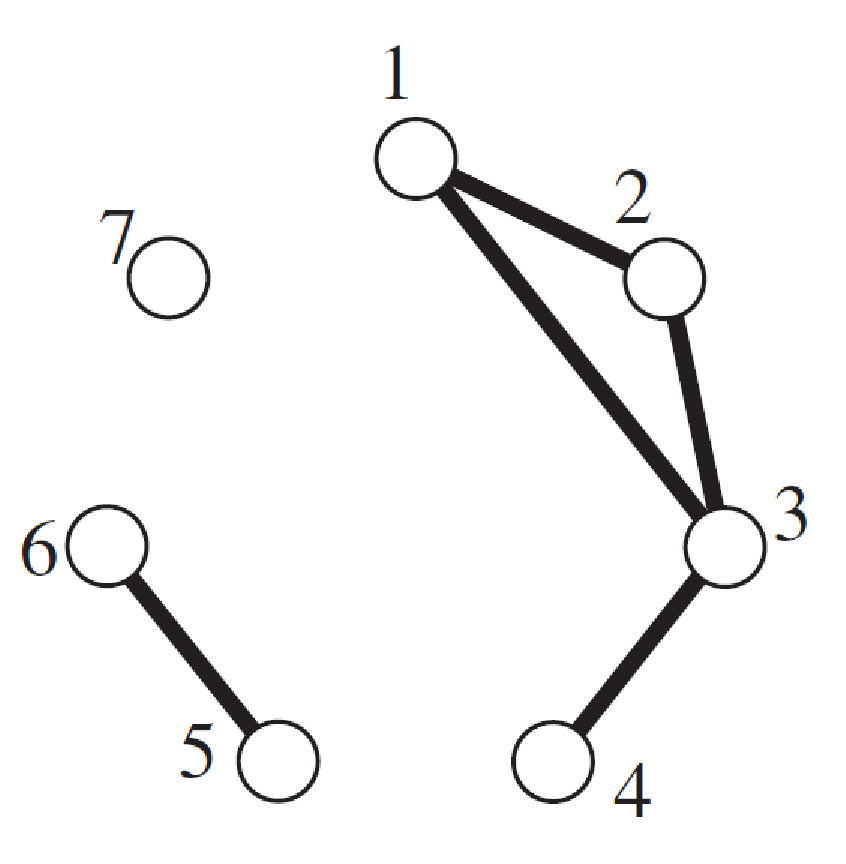
\includegraphics[scale=0.2]{Example1Visual.pdf}
\column{0.7\textwidth}
\[
\begin{array}{llll}
N(1)=\{2,3\}&N(2)=\{1,3\}\\
N(3)=\{1,2,4\}& N(4)=\{3\}\\
N(5)=\{6\}& N(6)=\{5\}\\
 N(7)=\emptyset
\end{array}
\]
\end{columns}
\end{frame}


\begin{frame}{Degree of vertices}
\bl[Definition]{
Let $G=(V,E)$ be a graph and let $v\in V$. The degree of $v$ is the number of edges with which $v$ is incident. The degree of $v$ is denoted $d_G(v)$ or, if there is no risk of confusion, simply $d(v)$.
}
\begin{columns}
\column{0.3\textwidth}

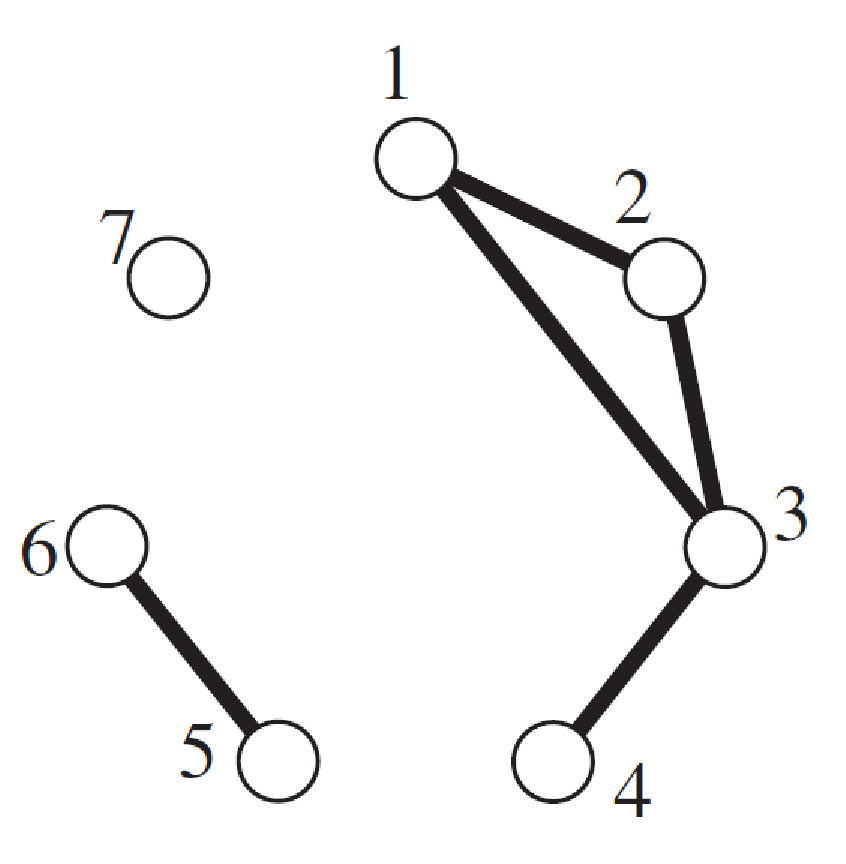
\includegraphics[scale=0.2]{Example1Visual.pdf}
\column{0.7\textwidth}
\[
\begin{array}{llll}
d(1)=2&d(2)=2&d(3)=3& d(4)=1\\
d(5)=1& d(6)=1& d(7)=0
\end{array}
\]
\end{columns}
Note that
\itemb
\item $d(v)=|N(v)|$
\item In the example, $\sum_{v\in V}d(v)=10$ which is also $2|E|$.
\iteme
\end{frame}

\begin{frame}
\bl[Theorem]{Let $G=(V,E)$. The sum of the degrees of the vertices in $G$ is twice the number of edges; that is,
\[
\sum_{v\in V}d(v)=2|E|
\]}
Suppose the vertex set is $\{v_1,v_2,\dots,v_n\}$. Consider the rectangular array where the $i,j$ entry is $1$ if $v_{i}\sim v_j$ and $0$ otherwise. In our example,
\begin{columns}
\column{0.5\textwidth}
\[
\left[\begin{array}{ccccccc}
0&1&1&0&0&0&0\\
1&0&1&0&0&0&0\\
1&1&0&1&0&0&0\\
0&0&1&0&0&0&0\\
0&0&0&0&0&1&0\\
0&0&0&0&1&0&0\\
0&0&0&0&0&0&0
\end{array}\right]
\]
\column{0.5\textwidth}
This is the \textbf{adjacency matrix} of the graph.
\end{columns}
\end{frame}

\begin{frame}
\bl[Theorem]{Let $G=(V,E)$. The sum of the degrees of the vertices in $G$ is twice the number of edges; that is,
\[
\sum_{v\in V}d(v)=2|E|
\]}
Consider the rectangular array where the $i,j$ entry is $1$ if $v_{i}\sim v_j$ and $0$ otherwise.\vspace{0.2cm}

\textbf{Q}: How many ones are in the adjacency matrix?
\itemb
\item For each $e\in E$, there are exactly two $1$-s in the matrix. Indeed, if $v_iv_j\in E$ then there is a $1$ at $ij$ and at $ji$. So one answer is $2|E|$.
\item In row $i$, there is a $1$ for every vertex adjacent to $v_i$. That is, the total number of $1$-s in row $i$ is $d(i)$. Therefore the second answer is $\sum_{v\in B}d(v)$.\qed
\iteme
\end{frame}

\begin{frame}{Further notation}
\itemb
\item \textbf{Maximum and minimum degree:} The maximum and minimum degree of a vertex in $G$ is denoted by $\Delta(G)$ and $\delta(G)$ respectively.
\item If all vertices in $G$ have the same degree $r$, we call $G$ $r$-regular.
\begin{figure}
\centering
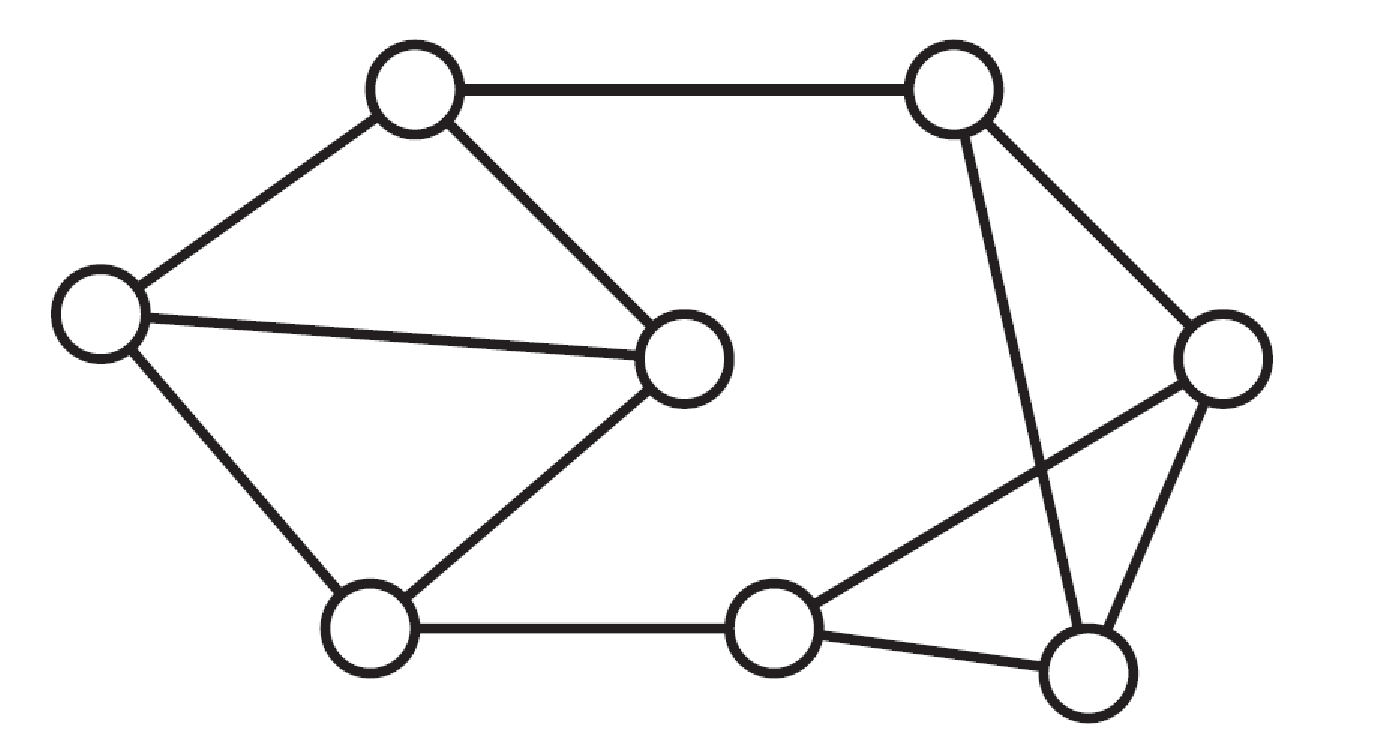
\includegraphics[scale=0.15]{Regular.pdf}
\end{figure}
\item The \textbf{order} of $G$ is $|V|$. The size of $G$ is $|E|$.
\item When the vertex and edge sets are not named, we will refer to them as $V(G)$ and $E(G)$.
\item We call $G$ a \textbf{complete graph} if all pairs of distinct vertices are adjacent. A complete graph of $n$ vertices: $K_n$.
\iteme
\end{frame}

\section{Subgraphs}

\begin{frame}
\bl[Definition]{Let $G$ and $H$ be graphs. We call $G$ a \textbf{subgraph} of $H$ provided $V(G)\subseteq V(H)$ and $E(G)\subseteq E(H)$.}
For example,\vspace{-0.3cm}
\begin{columns}
\column{0.5\textwidth}\vspace{0.1cm}
\[
V(G)=\{1,2,3,4,6,7,8\}
\]\vspace{-1.5cm}\\
\begin{align*}
~~~~~E(G)=&\big\{\{1,2\},\{2,3\},\{2,6\},\\
&\{3,6\},\{4,7\},\{6,8\},\\
&\{7,8\}\big\}
\end{align*}\vspace{-0.5cm}
\begin{figure}
\centering
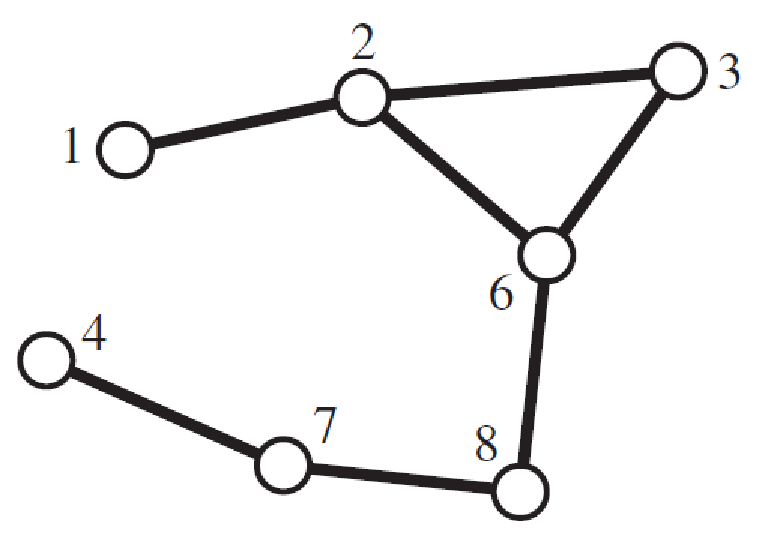
\includegraphics[scale=0.3]{subgraphexample1.pdf}
\end{figure}
\column{0.5\textwidth}
\[
V(G)=\{1,2,3,4,6,7,8,9\}
\]\vspace{-1cm}
\begin{align*}
~~~E(G)=&\big\{\{1,2\},\{1,4\},\{2,3\},\{2,5\},\\
&\{2,6\},\{3,6\},\{3,9\},\{4,7\}\\
&\{5,6\},\{5,7\},\{6,8\},\{6,9\}\\
&\{7,8\},\{8,9\}\big\}
\end{align*}\vspace{-1cm}
\begin{figure}
\centering
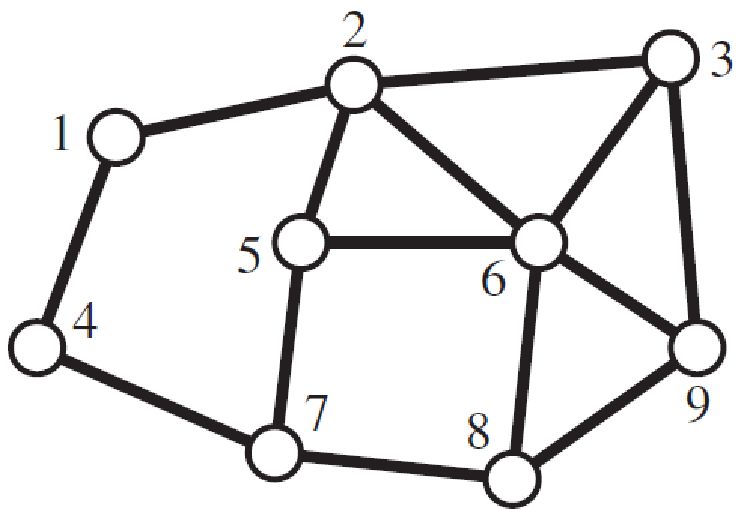
\includegraphics[scale=0.3]{subgraphexample2.pdf}
\end{figure}
\end{columns}
\end{frame}

\begin{frame}{Spanning subgraphs}
One way to get subgraphs is to delete edges. Let $H$ be a graph, then deleting the edge $e\in E(H)$, we get the graph $H-e$ which formally is the graph
\[
V(H-e)=V(H),\qquad E(H-e)=E(H)-\{e\}
\]
If we only remove edges, we get a spanning subgraph.
\bl[Definition]{Let $G$ and $H$ be graphs. We call $G$ a \textbf{spanning subgraph} of $H$ provided $G$ is a subgraph of $H$ and $V(G)=V(H)$.}\vspace{-0.2cm}
\begin{figure}
\centering
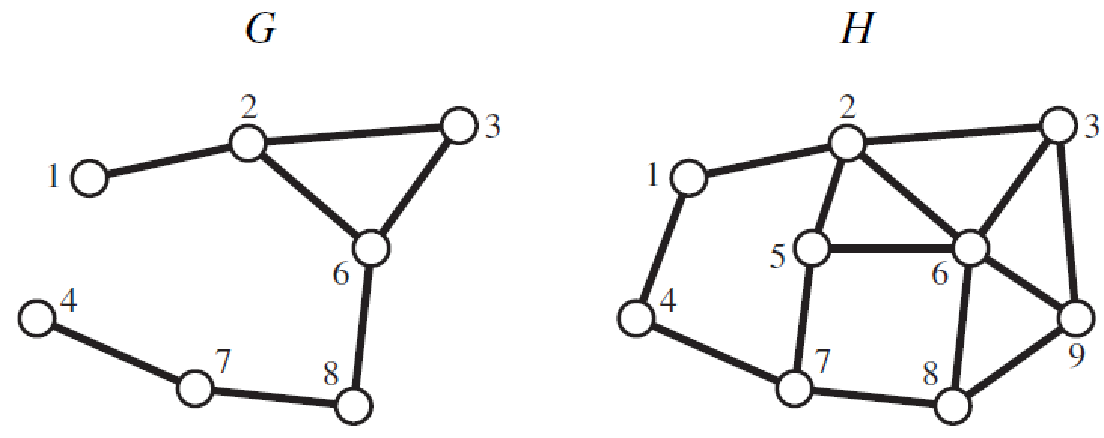
\includegraphics[scale=0.4]{SpanningSubgraph.pdf}
\end{figure}
\end{frame}

\begin{frame}{Induced subgraphs}
When removing a vertex $v\in V(H)$, we need to be more careful as we have to remove all the edges that $v$ is incident on.
\[
V(H-v)=V(H)-\{v\}\qquad E(H-v)=\{e\in E(H): v\notin e\}
\]
If we only remove vertices, we get an induced subgraph.
\bl[Definition]{Let $H$ be a graph and let $A$ be a subset of the vertices of $H$; that is, $A\subseteq V(H)$. The \textbf{subgraph of $H$ induced on $A$} is the graph $H[A]$ defined by
\[
V(H[A])=A,\qquad E(H[A])=\{xy\in E(H): x\in A, y\in A\}.
\]}
\end{frame}

\begin{frame}{Induced subgraphs}
In our earlier example, if $A=\{1,2,3,5,6,7,8\}$,
\begin{figure}
\centering
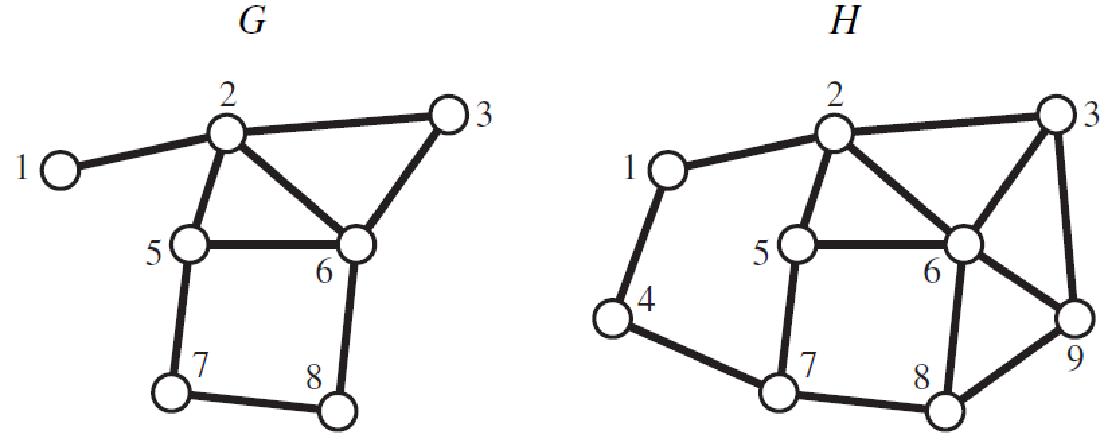
\includegraphics[scale=0.4]{InducedSubgraph.pdf}
\end{figure}
where $G=H[A]$.
\center Do Problem 3 on the worksheet.
\end{frame}

\begin{frame}{Cliques}
Subgraphs that are complete graphs have a special name.
\bl[Definition]{Let $G$ be a graph. A subset of vertices $S\subseteq V(G)$ is called a \textbf{clique} provided any two distinct vertices in $S$ are adjacent. The \textbf{clique number} of $G$ is the size of a largest clique; it is denoted by $\omega(G)$.}
In other words a set $S\subseteq V(G)$ is a clique provided $G[S]$ is a complete graph.
\begin{columns}
\column{0.4\textwidth}
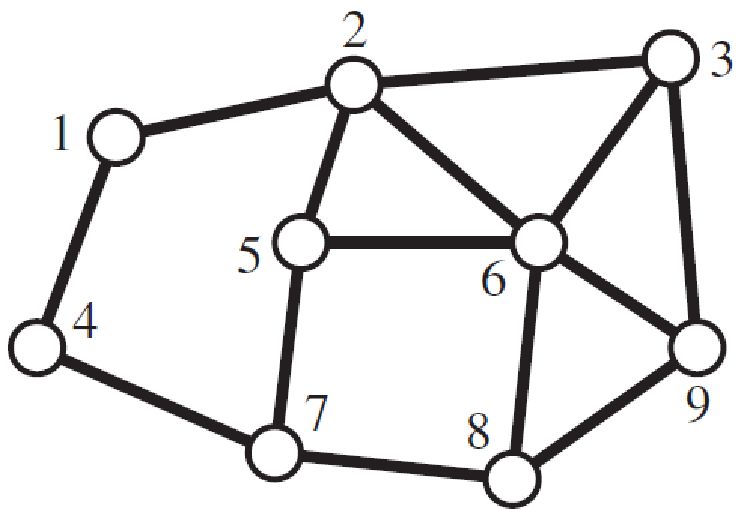
\includegraphics[scale=0.3]{subgraphexample2.pdf}
\column{0.6\textwidth}
Some of the cliques:
\[
\{1,4\}\qquad\{2,5,6\}\qquad \{9\}\qquad\{2,3,6\}
\]
\[
\{6,8,9\}\qquad\{4\}\qquad\emptyset
\]
We also have $\omega(H)=3$.
\end{columns}
\end{frame}

\begin{frame}{Independent sets}
Edgeless induced graphs also have a special name.
\bl[Definition]{ Let $G$ be a graph. A subset of vertices $S\subseteq V(G)$ is called an \textbf{independent set} provided no two vertices in $S$ are adjacent. The \textbf{independence number of $G$} is the size of a largest independent set; it is denoted $\alpha(G)$.}
In other words, a set $S\subseteq V(G)$ is independent if $G[S]$ is an edgeless graph.
\begin{columns}
\column{0.4\textwidth}
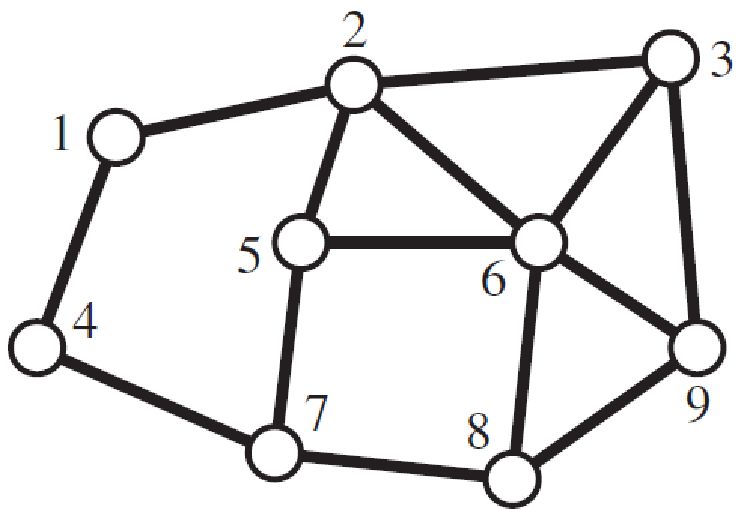
\includegraphics[scale=0.3]{subgraphexample2.pdf}
\column{0.6\textwidth}
Some of the independent sets:
\[
\{1,3,5\}\qquad\{1,7,9\}\qquad \{4\}\qquad\{4,6\}
\]
\[
\{1,3,5,8\}\qquad\{1,3,7\}\qquad\emptyset
\]
We also have $\alpha(H)=4$.
\end{columns}
\end{frame}

\begin{frame}{Complements}
Cliques and Independets sets are flipsides of the same coin.
\bl[Definition]{Let $G$ be a graph. The complement of $G$ is the graph denoted $\bar{G}$ defined by 
\[
V(\bar{G})=V(G),\qquad E(\bar{G})=\{xy:x,y\in V(G), x\neq y, xy\notin E(G)\}
\]}
In other words the complement is formed by removing all the edges from $G$ and replacing them by all possible edges that are not in $G$.\vspace{-0.3cm}
\begin{figure}
\centering
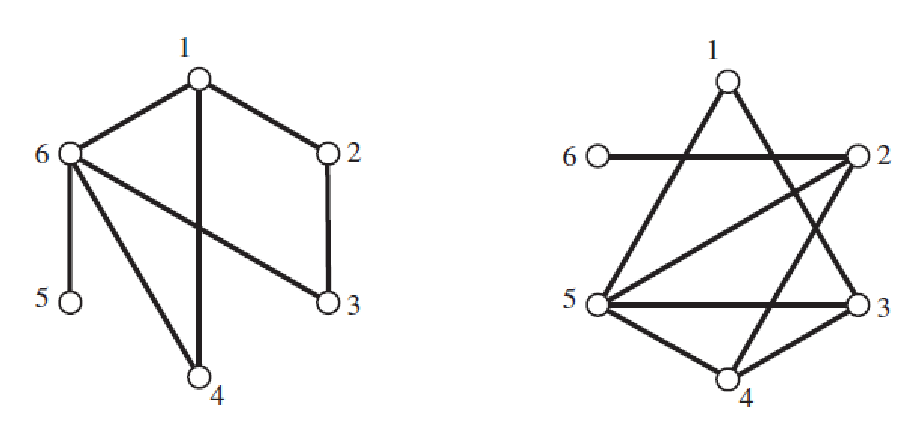
\includegraphics[scale=0.4]{Complements.pdf}
\end{figure}
\end{frame}

\begin{frame}{Cliques, independent sets in complementing graphs}
\bl[Proposition]{Let $G$ be a graph. A subset of $V(G)$ is a clique of $G$ if and only if it is an independent set of $\bar{G}$. Furthermore,
\[
\omega(G)=\alpha(\bar{G}),\qquad \alpha(G)=\omega(\bar{G})
\]}
\begin{center}
Do Problem 4-5!
\end{center}
\end{frame}
\end{document}